% The three strategists in the results: the archivist's four rules, the same without its
% evade rule, and the engage role alone. Wins against the yardstick are from
% `lab versus 200 <strategist> yardstick` (crates/lab), seeds 0-199, strategist in seat 0.
% Standalone: compiles on its own in Overleaf with pdflatex.
\documentclass[tikz,border=4pt]{standalone}
\usetikzlibrary{arrows.meta,shapes.geometric,positioning,calc}

% --- Colors: the deck's palette --------------------------------------------
\definecolor{paper}{HTML}{FDFDFC}   % node fill
\definecolor{ink}{HTML}{1B2430}     % text and edges
\definecolor{muted}{HTML}{6B7680}   % removed rules
\definecolor{act}{HTML}{2A6B4A}     % moves
\definecolor{intr}{HTML}{8B2E2E}    % interrupts

% --- Layout, in centimetres --------------------------------------------------
\newcommand{\TreeGap}{9.6}     % distance between the three trees
\newcommand{\LeafGap}{2.3}     % distance between leaves within a tree
\newcommand{\LeafY}{-2.4}      % height of the leaves
\newcommand{\BarMax}{6.0}      % bar length for 200 wins of 200
\newcommand{\BarY}{-4.9}       % height of the result bars

\begin{document}
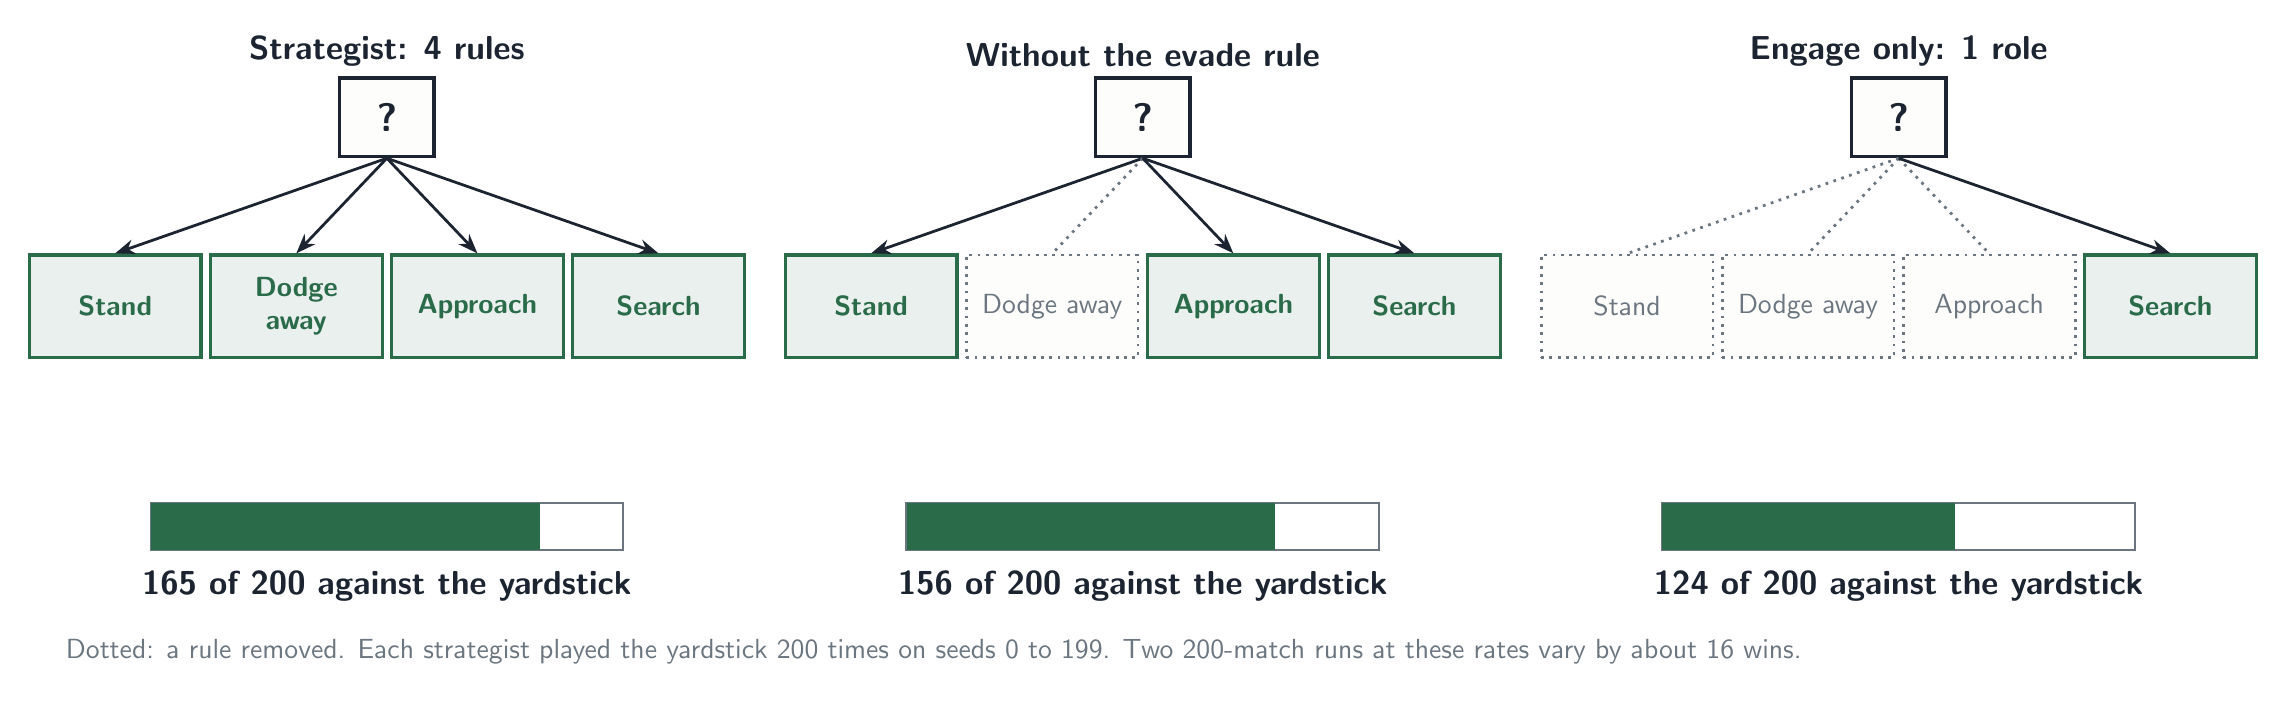
\begin{tikzpicture}[
    font=\sffamily\large, ink,
    edge/.style={-{Stealth[length=2.5mm]}, line width=1pt, draw=ink},
    selector/.style={draw=ink, line width=1.2pt, fill=paper, minimum width=1.2cm, minimum height=1cm, font=\sffamily\bfseries\Large},
    leaf/.style={draw=act, line width=1.2pt, fill=act!10, text=act, text width=1.9cm, align=center, inner sep=4pt, font=\sffamily\normalsize\bfseries, minimum height=1.3cm},
    leaf-edge/.style={edge},
    gone-edge/.style={-, line width=1pt, draw=muted, dotted},
    gone/.style={draw=muted, line width=1pt, dotted, fill=paper, text=muted, text width=1.9cm, align=center, inner sep=4pt, font=\sffamily\normalsize, minimum height=1.3cm},
  ]

% Each tree: its name, its wins against the yardstick, and its four leaves in rule order.
% A leaf style of "gone" marks a rule removed for the ablation.
\foreach \n/\name/\wins/\sa/\sb/\sc/\sd in {
    0/{Strategist: 4 rules}/165/leaf/leaf/leaf/leaf,
    1/{Without the evade rule}/156/leaf/gone/leaf/leaf,
    2/{Engage only: 1 role}/124/gone/gone/gone/leaf} {
  \pgfmathsetmacro{\cx}{\n*\TreeGap}
  \node[selector] (root\n) at (\cx, 0) {?};
  \node[anchor=south, font=\sffamily\bfseries\large] at (root\n.north) {\name};
  \foreach \k/\label/\st in {0/{Stand}/\sa, 1/{Dodge away}/\sb, 2/{Approach}/\sc, 3/{Search}/\sd} {
    \node[\st] (l\n\k) at (\cx + \k*\LeafGap - 1.5*\LeafGap, \LeafY) {\label};
    \draw[\st-edge] (root\n.south) -- (l\n\k.north);
  }
  % Against the yardstick: a bar out of 200.
  \draw[muted, line width=0.8pt] (\cx - \BarMax/2, \BarY) rectangle (\cx + \BarMax/2, \BarY - 0.6);
  \fill[act] (\cx - \BarMax/2, \BarY) rectangle (\cx - \BarMax/2 + \BarMax*\wins/200, \BarY - 0.6);
  \node[anchor=north, font=\sffamily\large\bfseries] at (\cx, \BarY - 0.75) {\wins{} of 200 against the yardstick};
}
\node[anchor=north west, text=muted, font=\sffamily\normalsize, align=left] at (-4.2, \BarY - 1.6)
  {Dotted: a rule removed. Each strategist played the yardstick 200 times on seeds 0 to 199. Two 200-match runs at these rates vary by about 16 wins.};

\end{tikzpicture}
\end{document}

% --- Self-check ----------------------------------------------------------------
% Trees: the archivist's rules (data/pilots.json) in order; the ablations remove the
%   dodge_away rule, and every rule but search, as in the deck's Method slide.
% Wins: 165, 156, 124 of 200, from lab versus against the yardstick (the deck's Results).
% Edges: a removed rule's edge is dotted and has no arrow (gone-edge).
% Bars: \BarMax is 200 wins; each bar is \BarMax x wins / 200.
% Noise: two standard errors of a difference of two 200-match rates near 80% is about
%   2 x sqrt(2 x 0.8 x 0.2 / 200) x 200 = 16 wins.
